\textnormal{
The user interface for this system is a simple-to-use desktop application. The system is initiated by clicking on the application icon on the user's machine. This will be followed by the main screen that allows to select the type of user interacting with the system. The following screen will be drawn up respective to the type of user selected in the previous screen.
}
\begin{figure}
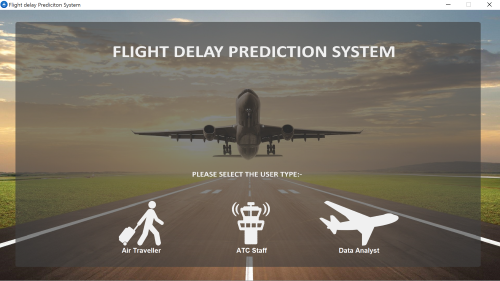
\includegraphics[width=\linewidth]{mainscreen.png}
\caption{Main screen of the application.}
\end{figure}
\begin{itemize} 
\item{User Interface screens and the flow of the application are as below:-}
\begin{itemize} 
\item{Fig. 4. shows the main screen that appears at the start of the application. The three options to the user are to select the user type that can be accessed by mouse click.} 

\item{Fig. 5. shows the input screen for the Air Traveller or the ATC Staff users. Note that the inputs required for both these users are the same. The inputs required here are in the drop down boxes next to their respective labels.}
\end{itemize}
\begin{figure}
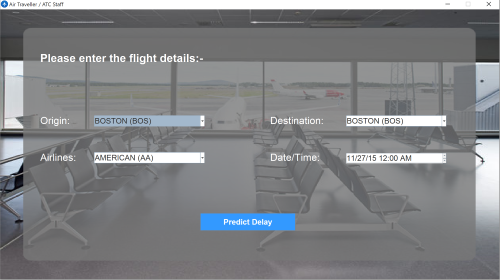
\includegraphics[width=\linewidth]{secondscreen.png}
\caption{User Input screen of the application.}
\end{figure}
\item{Information/Result messages displayed after user interaction are as below:-}
\begin{figure}
\centerline{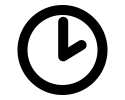
\includegraphics{delay.png}}
\caption{Dialog Box displayed when flight is predicted to be delayed.}
\end{figure}
\begin{figure}
\centerline{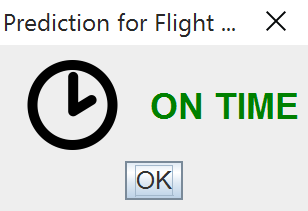
\includegraphics{ontime.png}}
\caption{Dialog Box displayed when flight is predicted to be on time.}
\end{figure}
\begin{itemize}
\item{Fig. 6. and Fig. 7. show the possible outcomes' dialog box when the user presses the predict button in the input screen.}
\end{itemize}
\item{Error messages shown for wrong user inputs are as below:-}
\begin{itemize}
\item{Fig. 8. shows the error message box that appears when the user inputs are such that the origin and the destination of the flights are kept the same.}
\item{The error in the Date/Time field is not shown on the screen but the default value for this field is taken as the input. This is because of the default inbuilt nature of the input field.}

\item{ The error messages in response to data range constraints violations.}
\begin{figure}
\centerline{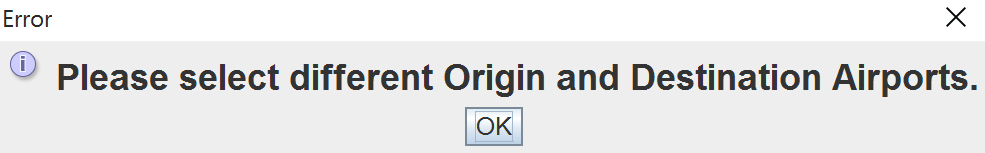
\includegraphics[width=\linewidth]{error.png}}
\caption{Error dialog for wrong user input.}
\end{figure}	
\end{itemize}
\end{itemize}


